% Extended chemical capacitance matrix C^ext as a star: every carrier node
% couples through a capacitor to a central phi node (the ideal case is a pure
% star). The nonideal direct carrier-carrier couplings are drawn dashed.
\documentclass[tikz, border=4pt]{standalone}
\usepackage[american]{circuitikz}

\begin{document}
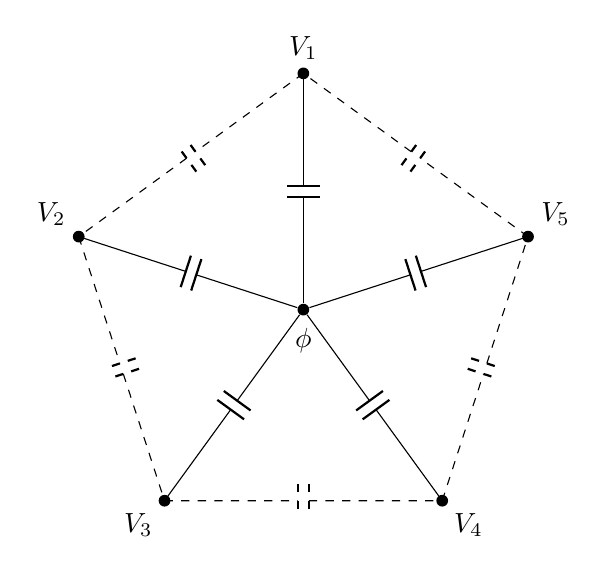
\begin{tikzpicture}
  \ctikzset{bipoles/length=0.7cm}

  % central phi node
  \node[circle, fill, inner sep=1.5pt, label={[label distance=1pt]-90:$\phi$}] (C) at (0,0) {};

  % 5 carrier nodes on a pentagon
  \foreach \i in {1,...,5} {
    \coordinate (N\i) at ({72 * (\i - 1) + 90}: 3);
    \node[circle, fill, inner sep=1.5pt,
          label={[label distance=-1pt]{72 * (\i - 1) + 90}:$V_{\i}$}] at (N\i) {};
  }

  % ideal star: each carrier capacitor-coupled to phi (solid)
  \foreach \i in {1,...,5} {
    \draw (N\i) to[C] (C);
  }

  % nonideal extras: direct carrier-carrier couplings (dashed perimeter)
  \foreach \i in {1,...,5} {
    \pgfmathtruncatemacro{\j}{mod(\i, 5) + 1}
    \draw[dashed] (N\i) to[C] (N\j);
  }
\end{tikzpicture}
\end{document}
